%!TEX root = ../gronskiy_phd_thesis.tex
\chapter[Minimum Spanning Tree Algorithms: Regularization by Stopping]{Minimum Spanning Tree
  Algorithms: \\ Regularization by Stopping}
\label{ch:mst}

\hfill
\begin{minipage}[t]{.75\textwidth}
\textit{``Besser ein Spatz in der Hand, als eine Taube auf dem Dach.'' \\
  (germ. ``A bird in the hand is worth two in the bush.'')} \\
  \hrule
  \vspace{.2cm}
  \hfill
  \textsc{--- Proverbs}
\end{minipage}

\section{Introduction}

\subsection{Motivation and Examples} 

\index{Minimum Spanning Tree}
\index{MST|see{Minimum Spanning Tree}}
Noise perturbed combinatorial optimization problems arise in various real-world
applications where problem instances are abstracted by weighted\footnote{We will
further utilize both the terms ``costs'' and ``weights'' in the same meaning.}
graphs with fluctuations in the weights. In this chapter, we
investigate the noisy Minimum Spanning Tree (MST) problems and their ability to
infer robust spanning trees. Examples of real-world applications of minimum
spanning trees come from various fields of human activity, such as
\emph{communication networks with delays} (optimizing message delivery times,
cf.~\citep{Bertsekas:1987}) or \emph{stock markets} (analyzing stock exchange
correlations, cf.~\citep{Sandoval:2012}), etc. All the applications require
trees with a high level of robustness to fluctuations since the quality of trees
is measured by expected costs. Wide real-world demand and applicability
stimulated extensive research on the robust minimum spanning trees
problem~\citep{Aron:2004, Kozina:1994, Sandoval:2012, Yaman:Karasan:Pinar:2001},
which addressed different aspects of the robust spanning tree setting, such as
development of algorithms, measuring algorithmic complexity, or comparing
robustness criteria.

In this chapter, we use an information-theoretic regularization approach
introduced in Chapter~\ref{ch:gen_appch} to analyse and validate MST algorithms
from the point of view of how well they can recognize (localize) the true
Minimum Spanning Tree under unknown noise in the graph instance. The validation
concept is developed for ``contractive'' algorithms that follow a step-by-step
strategy of shrinking the solution space until a single best solution is
identified.  This validation approach is based on the \emph{two-instance
scenario} \citep{Vapnik:1982} that requires statistical estimates to generalize
to test instances when the estimates have been inferred from a training
instance. For spanning trees, that means that they have to yield low costs on at
least two problem instances without being explicitly adapted to the test
instance.%%% JB: the reference to the IB method is obscure. We should
%%% reformulate it. 
Such regularization remains in the spirit of the \emph{information bottleneck
method}~\citep{Tishby:1999} in the sense that it tries to optimize the amount of
information that the algorithm might transfer from an artificial channel (see
below, Section~\ref{sec:ASReg}).
\index{Infromation bottleneck method}

%Suppose we need to construct a delivery
%network with minimal travel time along a given transportation system,
%where travel times along each road section fluctuate due to random
%transport delays caused by possibly unforeseeable events. Another 
%real-world application arises from stock financial markets,
%which exhibit strong correlations that can be
%modeled by a temporally evolving dependency graph. A minimalistic
%description of these correlations with a simple conditional
%independence structure requires to find a minimum spanning tree in
%such a noise contaminated graph (see~\citep{Sandoval:2012}). Both
%applications 

\subsection{Contributions and Outline of the Chapter}
\label{sec:mst_contribs}
As main contributions of this chapter, we
\begin{itemize}
  \item define a notion of contractive algorithm and give an general
  extension of the ASC regularization approach (introduced earlier in
  Chapter~\ref{ch:gen_appch}) for the case of stepwise contractive algorithmic
  problems. We call it Algorithmic ASC;
  \item provide a specialization of such extension to the case of three major
  algorithms solving the Minimum Spanning Tree (MST) problem, including the
  necessary tools to avoid brute-force enumeration known as a computational
  bottleneck of ASC;
  \item carry out experiments which justify usage of Algorithmic ASC score as
  a ranking tool related to expected localization error: higher Algorithmic ASC
  score yields lower error.
\end{itemize}

The chapter is outlined as follows. First, a related work overview is given in
Section~\ref{sec:mst_related_work}. Then, in Section~\ref{sec:mst_related_work}
we revisit those ingredients of ASC approach relevant for this chapter. A
comprehensive introduction into the original approximation set-based approach is
then given in Section~\ref{sec:asc_original}. Later, the main contribution is
made in Section~\ref{sec:mst_algorithmic_gen}, where we make a generalization of
the ASC to algorithmic problems, and Section~\ref{sec:applying_asc_to_mst} where
we directly apply it to Minimum Spanning Tree (MST) problem and three most
important algorithms solving it. Experimental results follow in
Section~\ref{sec:mst_results}. Finally, we discuss our findings in
Section~\ref{sec:mst_conclusion}.

\section{Related Work Overview} 
\label{sec:mst_related_work}

Literature entries on robust spanning trees vary by research purpose
(e.g.~algorithm complexity, robustness), adopted noise model
(e.g.~interval data), regularization strategy (regularizing by
pruning, graph preprocessing).  For example,
\citep{Yaman:Karasan:Pinar:2001} investigated graphs with edge weights
which are supposed to fall uniformly into a predefined interval. The
approach is based on regularization \emph{by preprocessing the graph},
which, in turn, involves eliminating selected edges and forcing other
edges to be included into the spanning tree.

\index{Pruning (tree)}
Regularizing an MST by \emph{pruning} as proposed
by~\citep{Sandoval:2012} identifies the presumably robust part of a
spanning tree. This goal is achieved by means of analyzing the
survival matrix constructed from adjacency matrices for training
minimum spanning trees.

Our approach is similar in that pruning (more precisely, optimal
stopping) is used as a regularization tool, but it rather aims at
\emph{analysis and comparison} of the algorithm's robustness by means
of such regularization. This approach also exhibits technical
differences from the mentioned work, relying only on \emph{two} data
instances, and it follows the spirit of learning theory with its goal
to analyse algorithms in a noise distribution independent way.

In Section~\ref{regularization_gen}, the general concepts of the
information-theoretic framework are given, as well as the
information-theoretic motivation. Then, in
Section~\ref{sec:mst_algorithmic_gen}, the application to stepwise algorithms
is discussed. The results and conclusion are summarized in
Sections~\ref{sec:mst_results} and~\ref{sec:mst_conclusion}, respectively.

\section{Approximation Set Coding Regularization}
\label{regularization_gen}

To make this chapter self-consistent, we first give a short overview of the approach
first introduced in Chapter~\ref{ch:gen_appch}, as well as of the
notation and terms used throughout this chapter.
\index{Regularization}

\subsection{Notation and Definitions}

Assume, there is a data instance $X$ given, for example
measurements in a data space $\mathcal{X}$, so that $X \in
\mathcal{X}$. In case of the MST problem, $\mathcal{X}$ is the set of
all possible combinations of the edge costs and $X$ is a particular realization
of such costs. Let $c$ denote a solution in a general set of solutions $\C$, so
that $c \in \C$. In case of the MST, $\C$ is the set of feasible spanning trees.

An optimization problem is defined by a cost (objective) function $R:
\C\times\mathcal{X}\rightarrow \mathbb{R}_{+}$ that assigns
each solution $c$ a real value $R(c,X)$. Furthermore,
$c^{\bot}(X) \in \arg\min_{c \in \C} R(c, X)$
denotes\footnote{In the context where it is clear what $X$ is, we
will omit the ``$(X)$'' in the notation: $c^\bot(X) \equiv
c^\bot$; $R(c,X) \equiv R(c)$; $\C_\gamma(X) \equiv
\C_\gamma$.} the minimum cost solution.

For the sake of referring to it in the rest of the chapter, we give here a
definition from Chapter~\ref{ch:gen_appch}:
\begin{definition}
\label{def:mst_ch_approximation_set}
For a given real number $\gamma \ge 0$, an approximation set is defined as follows:
\begin{equation}
  \mathcal{C}_\gamma (X, R) \coloneqq 
  \{c \in \mathcal{C} \mid R(c, X) - R^\bot(X) \le \gamma\},
\end{equation}
\end{definition}

In fact, it is desirable to find a \emph{robust set} of solutions
rather than a single solution, since we cannot trust the global
minimizer $c^\bot$ to achieve low costs on test instance due to noise
in the measurements. In this light, the sets $\C_\gamma(X)$ play
the role of a ``trade-off agent'' in the process of finding the robust
solution to optimization problem. This trade-off is 
%%% meant to be the one 
balancing the solution sets between overfitting ($\gamma = 0$) and underfitting (large
$\gamma$).
\index{Global minimizer}
\index{Overfitting}
\index{Underfitting}

%%%%%%%%%%%%%%%%% JB corrections up to here %%%%%%%%%%%%%%%%%

\subsection{Robust Solving via ASC Regularization}
\label{subsec:asc_regularization_crit}
Regularization by the Approximation Sets applies to a situation, when two data
instances $X', X'' \in \mathcal{X}$ are available and when both are generated by
injecting two noise realizations into the true data instance $X^0 \in
\mathcal{X}$ (see Section~\ref{sec:data_generation_model}). It is required for
both cases that the noise follows the same noise distribution: $X', X'' \sim
PG(X^0)$. In the spirit of statistical learning theory, we are interested in
distribution independent results since the distribution $PG(X^0)$ might be
unknown.

A robust solution to the noisy optimization problem $(\mathcal{X}, \C, R)$ is
obtained by the two-step process described in
Algorithm~\ref{alg:robust_solving_via_similarity}.

\begin{algorithm}[hb!]
\caption{Robust Solving via ASC Regularization}
\label{alg:robust_solving_via_similarity}
  \KwData{\\
  \quad two instances of the $X', X''$, \\ \\ 
  \quad cost function $R(c, X)$}

  \KwResult{Solution $c \in \C$.}

  {
    Find the optimal regularization parameter $\gamma^*$ that
    maximizes the log-ratio 
    % involving \emph{the first two data instances}:
    \begin{equation}\label{eq:mst_asc_ratio}
      \hat I_\gamma(X', X'') \coloneqq \log 
      \Bigl(
        \frac{|\C| \; |{\C}_{\gamma}(X') \cap {\C}_{\gamma}(X'')|}%
          {|\mathcal{C}_\gamma(X')| \; |\mathcal{C}_\gamma(X'')|}
      \Bigr),
    \end{equation}
  }

  {Choose a solution uniformly at random from the intersection of
        optimal approximation sets: $c \in C_{\gamma^*}(X') \cap
        C_{\gamma^*}(X'')$.}
\end{algorithm}

\myremark Note the difference of~\eqref{eq:mst_asc_ratio} with previously
defined~\eqref{eq:asc_mutual_information_formula}: dropping the 
expectation. This is perfectly legitimate in case when we have no access to the
problem generation distribution and have to replace the actual value by its
estimator.

\subsection{Information-Theoretic Basis for ASC Regularization}
\label{sec:ASReg}

Applying of ASC bases itself on the information-theoretic ground which uses
approximation sets $\C_{\gamma}(X)$ in a fictitious communication scenario.
This communication scenario involves sending and receiving a
\emph{transformation} $\tau\colon
\mathcal{X} \to \mathcal{X}$ that maps the data space onto
itself. We briefly recap the necessary information here: for a full
introduction, refer to Chapter~\ref{ch:gen_appch}
(Section~\ref{sec:communication_learning_stability}).

Communicating a true $\tau_{\mathrm{send}}$ is performed by sending ${\tau_{\mathrm{send}} \circ
X'}$ to the receiver, while the channel perturbs this ``message''
by substituting $X'$ with $X''$. Finally, the receiver obtains
$\tau_{\mathrm{send}} \circ X''$. The reader should note that $X'$ is known to
both sender and receiver.
\index{Sender}
\index{Receiver}
\index{Approximation Set Coding!Encoding and transmission}
\index{Approximation Set Coding!Decoding}

As the receiver 
%%% JB: receives
accepts $\tau_{\mathrm{send}} \circ X''$, it has has to distinguish the
fluctuations in $X''$ relative to $X'$ from the applied
transformation $\tau_{\mathrm{send}}$. Error free communication is guaranteed if the
receiver can identify the correct transformation $\tau_{\mathrm{send}}$ without
being deceived by these fluctuations.  The straightforward decoding
rule consists in finding the ``nearby'' transformation $\hat \tau$,
which maximizes the overlap between the received approximation set
$\C_\gamma(\tau_{\mathrm{send}} \circ X'')$ and the ``nearby'' approximation set
$\C_\gamma(\hat\tau \circ X')$.

The role of the codebook vectors is played by all such transformations
which enable us to cover the complete solution space $\C$
with approximation sets $\C_\gamma(\tau \circ X')$. Obviously,
$\gamma$ controls the number of such codebook vectors since for large
$\gamma$ we can only select few such sets to cover $\C$;
otherwise we risk decoding errors. The concept is analogous to
classical coding theory where every codebook vector defines the
``center'' of an ``error-correcting'' sphere, and the elements of this
sphere are \emph{indistinguishable} from the data transmission point
of view.
\index{Indistinguishable solutions|see{Solutions}}
\index{Solutions!Indistinguishable}

As derived in Section~\ref{sec:communication_learning_stability}, an
asymptotically vanishing error probability is achievable for coding rates
bounded by
%%
\begin{align}
  I_\gamma(X', X'') &= \Expct \hat I_\gamma(X', X'') \notag \\ 
  &=
  \Expct \log\left( \frac{|\C| \, |{\C}_{\gamma}(X') \cap
      {\C}_{\gamma}(X'')|}{|{\C}_{\gamma}(X')|
      \, |{\C}_{\gamma}(X'')|}\right), \label{eq:mst_ch_mutual_inf}
\end{align}
The estimator $\hat I_\gamma(X', X'')$ in (\ref{eq:mst_ch_mutual_inf}) measures
the total information content of a message.

For a fixed $\gamma$, a large overlap means that the evaluation of the first
dataset generalizes to the second dataset, whereas a small or empty intersection
indicates lack of generalization. The fraction of approximation set
cardinalities in (\ref{eq:mst_ch_mutual_inf}) measures stability of the solutions under
noise fluctuations.

The value $\Expct \hat I_{\gamma}(X', X'')$ is an estimate for the \emph{mutual
information} and, in analogy to information theory
(cf.~\citep[Ch.~7]{Cover:2006}), the \emph{approximation capacity} is defined as
$C \coloneqq\max_{\gamma}\Expct [\hat I_{\gamma}(X', X'')]$ (cf.
Definition~\ref{def:asc_score}). The expectation $\Expct$ is taken with respect
to the random variables $X', X''$. If the distribution $PG(X^0)$ is unknown then
we have to derive learning theoretic large deviation bounds based on the
empirical quantity $\hat I_{\gamma}(X', X'')$ and appropriate complexity
penalties.

In summary, maximizing the ratio~\eqref{eq:mst_asc_ratio} allows us to select the
optimal resolution for the solution set, and elements of this approximation set
are considered indistinguishable given the present noise process.

\section{ASC Regularization for Stepwise Algorithms}
\label{sec:mst_algorithmic_gen}

\subsection{Application to Stepwise Algorithms: Main Idea}

Direct application of ASC regularization requires
optimizing~\eqref{eq:mst_asc_ratio} w.r.t.~$\gamma$, which, in turn, amounts
to compute the cardinalities 
\begin{equation}
  |{\C}_{\gamma}(X') \cap {\C}_{\gamma}(X'')|, 
  \quad |{\C}_{\gamma}(X')|, 
  \quad |{\C}_{\gamma}(X'')|
\end{equation}
(cf. Definition~\ref{def:mst_ch_approximation_set}).  In general, computation or
at least estimation of these cardinalities requires to enumerate the elements of
$\C$ and to test if they belong to $\C_\gamma$. Such enumeration is
computationally hard, since $\C$ grows sometimes very fast (exponentially in
cases of some combinatorial problems).\footnote{This difficulty emerges as a
common bottleneck in many problem settings. We elaborated on it in
Section~\ref{sec:gen_appch_conclusion} of the previous chapter.}

For algorithms, these enumeration problems arise in a constraint form, i.e.,
\emph{the algorithm itself} might help to optimize this enumeration, eliminating
all those solutions that get ``out of consideration'' as the algorithm
progresses. In other words, some algorithms feature a step-by-step nature, and
they shrink the set of feasible solutions at each next step, ending up with the
optimal solution at the last step. Figure~\ref{fig:mst_contractive_algorithm}
illustrates this intuition. This contraction is very similar to the shrinkage of
approximation sets, as they shrink to the optimal solution as $\gamma$
decreases. The feasible sets induced by the algorithm often turn out to be
efficiently computable~-- and we will exploit this property of contractive
algorithms. 

\subsection{Contractive Algorithms and Their Approximation Sets}
\index{Contractive algorithm}We define the algorithmic approximation set at computational step $t$ as the set
of solutions that are still considered as potential answers to be returned by
the algorithm $\algo$. This generalized notion of an approximation set for
algorithm $\algo$ measures the statistical behavior of a specific algorithm
during its execution. 
\nomenclature[E, 05a]{$\algo$}{algorithm\nomnorefeq}%

\myremark Even if $\algo$ calculates the global minimum of the cost
function, the algorithm may not follow a gradient flow on that costs to
determine the global minimum.

\begin{figure}[ht!]
  \centering
  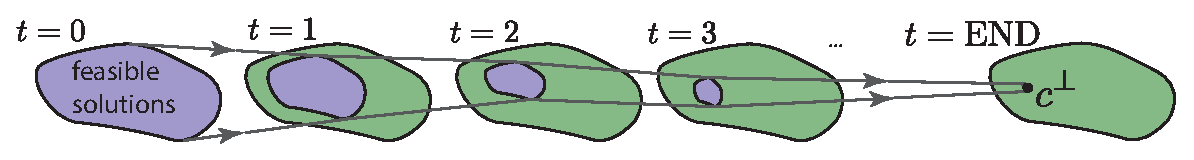
\includegraphics[width=\textwidth]{figures/ch_mst/contractive_alg}
  \\[.5cm]
  \caption{Illustration of a contractive algorithmic flow: the set of
    feasible (i.e. still possible) solutions contracts from step to step,
    shrinking to $c^\bot$ at the end of execution.}
  \label{fig:mst_contractive_algorithm}
\end{figure}

\begin{definition}
\label{def:contractive_algorithm}
  Assume that for a given data instance $X$ the stepwise execution of the
  algorithm $\algo$ evaluated on this instance can be expressed as a sequence of
  subsets of feasible solutions
  %%
  \begin{align}
    \algo(X) &= \langle A_0(X), \ldots, A_T(X)
    \rangle,
    \quad\text{where} \notag \\
  %%
    A_t(X) &\subseteq \C, \quad t = 0, \ldots, T, \qquad\quad
    \text{and} \notag\\
  %%
    A_0(X) &= \C \notag \\ 
    A_T(X) &= \{c^\bot\}.
  \end{align}
  \nomenclature[E, 05b]{$A_i(X)$}{algorithmic feasible set\mynomdef{def:contractive_algorithm}}%
  \nomenclature[E, 05b]{$T$}{total number of steps\nomnorefeq}%
  %%
  We call $\algo$ contractive, if $A_{t+1} \subseteq
  A_{t}$.  
\end{definition}

\begin{definition}\label{def:algorithmic_approximation_set}
  For a contractive algorithm it is natural to define an algorithmic
  $t$-approximation set as follows: $\C^\algo_t(X) \coloneqq A_t(X)$.
  \nomenclature[E, 05d]{$\C^\algo_t(X)$}{algorithmic $t$-approximation set\mynomdef{def:algorithmic_approximation_set}}%
  \index{Algorithmic!Approximation set}
  \index{Approximation set!Algorithmic|see{Algorithmic}}
\end{definition}

An example of such algorithm, as well as comprehensive illustration, will be
given in Section~\ref{sec:applying_asc_to_mst} and
Figure~\ref{fig:ch_mst_illustration}.

Speaking informally, the algorithmic $t$-approximation set is an approximation
set as defined in Definition~\ref{def:mst_ch_approximation_set}, but taken
w.r.t. the flow of a particular algorithm at update step $t$. The role of the
$\gamma$ parameter is now (in contrast to
Definition~\ref{def:mst_ch_approximation_set}) played by a discrete step
variable $t$ spanning from $0$ to $T$ (note that, generally, $T$ is not a
constant). All the other notions remain the same when adopting the new
definition of the approximation sets $A_t(X)$. For example, the following
defines the algorithmic ASC score:

\begin{definition}
As an analogy to~\eqref{eq:mst_ch_mutual_inf}, we will call the quantity
%%
\begin{align}\label{eq:alg_eq:mst_asc_ratio}
  I_t^\algo = \Expct \hat I_t^{\algo}( X', X'' ) 
    &\coloneqq \Expct \log\biggl( \frac{|\C| \, |{\C}^\algo_{t}(X') \cap
      {\C}^\algo_{t}(X'')|}{|{\C}^\algo_{t}(X')|
      \, |{\C}^\algo_{t}(X'')|}\biggr) \notag \\
    &\equiv \Expct \log \biggl(\frac{
      |\C|\; |A_t(X') \cap A_t(X'')|
    }{
      |A_t(X')|\; |A_t(X'')|
    }\biggr), 
\end{align}
\nomenclature[E, 05g]{$I_t^\algo$}{algorithmic ASC $t$-score}%
\nomenclature[E, 05ga]{$\hat I_t^\algo$}{empirical algorithmic ASC $t$-score}%
where $A_t(\cdot)$ are defined above, an algorithmic ASC $t$-score.
\index{Algorithmic!ASC score}
\index{Approximation Set Coding!Algorithmic|see{Algorithmic}}
\end{definition}
As in Chapter~\ref{ch:gen_appch}, we will distinguish between 
expected and empirical values.

\subsection{Algorithmic ASC Score and Optimal Stopping}
\begin{figure}[hb!]
  \centering
  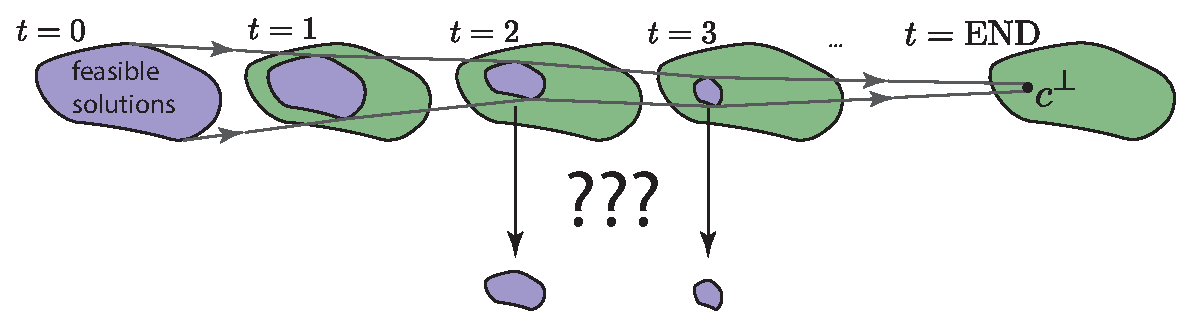
\includegraphics[width=\textwidth]{figures/ch_mst/contractive_alg_opt_stop}
  \\[.5cm]
  \caption{The main question addressed in this chapter: which of the steps to
    choose for the optimal stopping.}
  \label{fig:mst_contractive_algorithm_opt_stop}
\end{figure}
As an empirical extension of the notions introduced in
Chapter~\ref{ch:gen_appch}, we claim that the algorithmic channel capacity
\begin{equation}
  C^\algo \coloneqq \max_{t = [0, \ldots, T]} I^\algo_{t} 
    = \max_{t = [0, \ldots, T]}\Expct [\hat I^\algo_{t}(X', X'')],
\end{equation} 
\nomenclature[E, 05gb]{$C^\algo$}{algorithmic approximation capacity}%
also referred as~\emph{algorithmic approximation capacity} or \emph{information
content}, equals the maximum amount of information which could be transferred
through a fictitious channel described in Section~\ref{sec:ASReg} (and, in more
detail, earlier in Section~\ref{sec:communication_learning_stability}), and
constrained to the specific algorithm (i.e., algorithmic approximation sets are
allowed). From the learning perspective, the algorithmic approximation capacity
shows how well the algorithm can filter out the noise (by $t$-optimization),
remaining robust to underfitting.
\index{Algorithmic!Approximation capacity}
\index{Optimal stopping}

In a full analogy with the approach of Chapter~\ref{ch:gen_appch}
(cf.\eqref{eq:asc_best_gamma}), one can find the optimal stopping time $t^*$ by
maximizing the algorithmic ASC $t$-score:
\begin{equation}\label{eq:mst_asc_best_step}
  t^* \in \arg \max_{t = [0, \ldots, T]} \hat \Expct I^\algo_t(X', X'').
\end{equation}
\nomenclature[E, 05g]{$t^*$}{optimal stopping time}%
We are going to use this approach as an optimal stopping criterion for the 
rest of the chapter (see Figure~\ref{fig:mst_contractive_algorithm_opt_stop}).

\myremark We will call this approach \textit{algorithmic ASC} opposed to the
original ASC approach developed in Chapter~\ref{ch:gen_appch}.
\index{Algorithmic!Approximation Set Coding}

\section{ASC Regularization for MST Algorithms}
\label{sec:applying_asc_to_mst}

\subsection{Major MST Algorithms}
In the rest of the chapter, we will consider the Minimum Spanning Tree (MST)
problem. Its formulation is as follows: given a weighted undirected graph $G =
(V, E)$, find a spanning tree of the minimum possible weight. \textit{Spanning
tree} is defined as a connected subgraph of $G$ without cycles, whose vertex set
equals $V$.
\index{Tree!Spanning}
\index{Spanning tree|see{Tree}}

There are several classical solutions to this problem, of which we will focus on
\textit{Prim's}, \textit{Kruskal's} and \textit{reverse-delete} algorithms. We
bring their definitions in a pseudo-code in
Algorithms~\ref{alg:prim_alg_pseudocode},~\ref{alg:kruskal_alg_pseudocode}
and~\ref{alg:rd_alg_pseudocode} and explain a verbal intuition behind them below.
\index{MST Algorithm!Prim's}
\index{MST Algorithm!Kruskal's}
\index{MST Algorithm!Reverse-delete}
\index{Prim's|see{MST Algorithm}}
\index{Kruskal's|see{MST Algorithm}}
\index{Reverse-delete|see{MST Algorithm}}


\begin{algorithm}[ht!]
\caption{Prim's Algorithm for finding MST}\label{alg:prim_alg_pseudocode}
\KwIn{undirected graph $G(V, E)$ with non-negative weights}
\KwOut{spanning tree with minimum total weight}
{initialize current tree $B = (V_B, E_B)$ by choosing first vertex: 
  $B \leftarrow (\{v^*\}, \emptyset)$\;}

\While{$V_B \ne V$ (not all vertices are in tree)}{
  {find the minimal edge $e_\mathrm{min} = (v, v_\mathrm{min})$ 
    from $B$ to the rest $G \setminus B$\;} 
  {add $e_\mathrm{min}$ to the tree $B$\;} }

\KwRet{current tree $B$}
\end{algorithm}

\begin{algorithm}[ht!]
\caption{Kruskal's Algorithm for finding MST}\label{alg:kruskal_alg_pseudocode}
\KwIn{undirected graph $G(V, E)$ with non-negative weights}
\KwOut{spanning tree with minimum total weight}
{initialize current tree $B = (V_B, E_B)$: $B \leftarrow (\emptyset, \emptyset)$ \;}

\While{$V_T \ne V$ (not all vertices are in tree)}{
  {find the minimal edge $e_\mathrm{min}$ such that: \\
    \quad a) $e_\mathrm{min} \not \in E_B$ and \\ 
    \quad b) $B \cup e_\mathrm{min}$ has no cycles\;} 
  {add $e_\mathrm{min}$ to the tree $B$\;} 
}

\KwRet{current tree $B$}
\nomenclature[E, 10a]{$G(V, E)$}{graph\nomnorefeq}%
\end{algorithm}

\begin{algorithm}[ht!]
\caption{Reverse-Delete Algorithm for finding MST}\label{alg:rd_alg_pseudocode}
\KwIn{undirected graph $G(V, E)$ with non-negative weights}
\KwOut{spanning tree with minimum total weight}
{initialize current graph $B = (V_B, E_B)$ with the input graph: $B \leftarrow G$
\;}

\While{$B$ is connected and yet not a tree}{
  {find the maximal edge $e_\mathrm{max}$ in $B$ such that: \\
    \quad deleting $e_\mathrm{max} $ does not disconnect $B$\;} 
  \If{no such edge found}{break\;}
  \Else{remove $e_\mathrm{max}$ from $B$\;} 
}

\KwRet{current tree $B$}
\end{algorithm}

\begin{figure}[th!]
  \centering
  \begin{subfigure}[b]{.48\textwidth}
      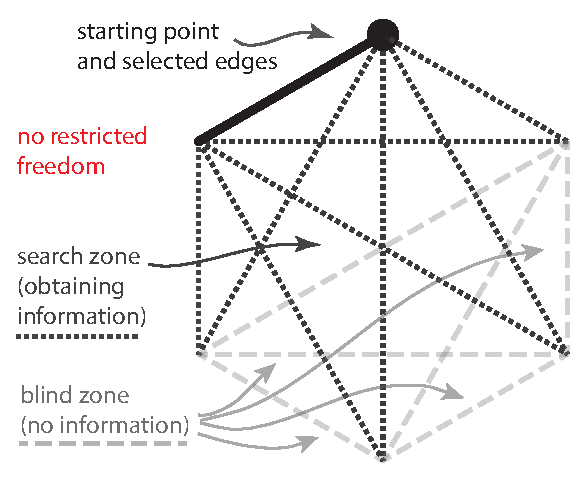
\includegraphics[width=\linewidth]{figures/ch_mst/mst_illustration_0}
      \caption{Step 2: candidate edges set is large, no restricted edges yet}
      \label{fig:ch_mst_illustration-0}
  \end{subfigure}
  \hfill
  \begin{subfigure}[b]{.48\textwidth}
      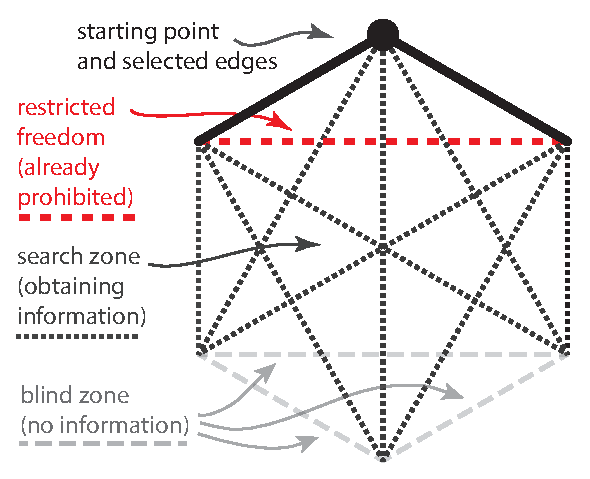
\includegraphics[width=\linewidth]{figures/ch_mst/mst_illustration_1}
      \caption{Step 3: candidate edges set is large gets smaller, restricted edges appear}
      \label{fig:ch_mst_illustration-1}
  \end{subfigure}
  \\[.5cm]
  \begin{subfigure}[b]{.48\textwidth}
      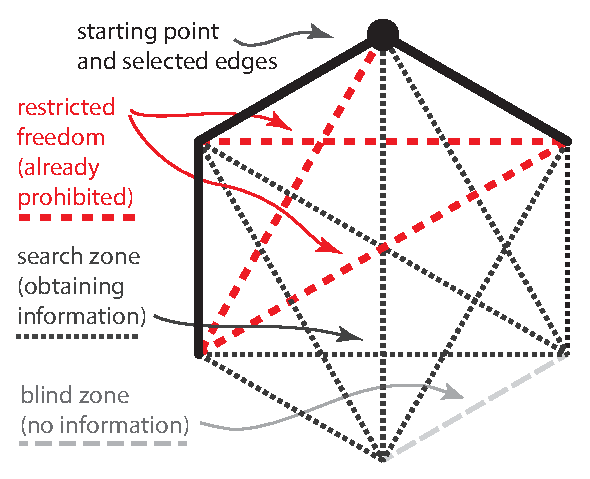
\includegraphics[width=\linewidth]{figures/ch_mst/mst_illustration_2}
      \caption{Step 4: candidate edges set is large gets even smaller, restricted edges build up}
      \label{fig:ch_mst_illustration-2}
  \end{subfigure}
  \hfill
  \begin{subfigure}[b]{.48\textwidth}
      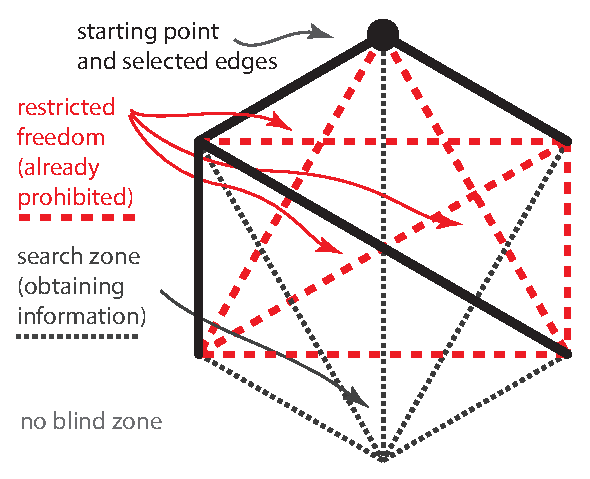
\includegraphics[width=\linewidth]{figures/ch_mst/mst_illustration_3}
      \caption{Step 5: almost everything is restricted}
      \label{fig:ch_mst_illustration-3}
  \end{subfigure}
  \\[.5cm]
  \caption{Prim's MST Algorithm: freedom reduces as information
    grows. Edge weights are not shown (figure from the introduction recreated
    here for convenience).}
  \label{fig:ch_mst_illustration}
\end{figure}

\emph{Prim's algorithm} (``growing tree'' strategy) starts with a tree $B=(V_B,
E_B)$ on an empty set of edges $E_P$ and a starting vertex $v^{*}$. The
algorithm enlarges $E_B$, adding one edge $e_t$ at step $t$ (the first step
adds an edge incident to $v^{*}$), so that $B$ remains to be a tree, until $B$
becomes a spanning tree of $G$. It takes $T = n-1$ steps.

\emph{Kruskal's algorithm} (``connecting trees in a forest'' strategy) of
finding MSTs starts with an empty set of edges $E_B$. The algorithm adds
a minimal possible $e_t$ at the step $t$, not allowing cycles in $E_B$,
but yet not requiring $B$ to be connected at all times, until $B$ becomes a spanning tree
of $G$. It takes $T = n-1$ steps.

\emph{Reverse-Delete} (``reducing graph'' strategy) algorithm starts
with a graph on the full set of edges $B = G$ and shrinks it, removing one maximal edge
$e_t$ per step and keeping the graph
$B$ connected, until $B$ becomes a spanning tree. 
For a complete graph, it takes $T = n(n-1)/2 - n + 1$ steps.

\myremark All the three algorithms can be easily proven to reach the global
minimizer solution $c^\bot(X) \in \arg \min_c R(c, X)$.

\subsection{Counting Approximation Sets for MST}

\paragraph{MST algorithms are contractive} From the description of three
algorithms in the previous section one can see, that they all comply with the
Definition~\ref{def:contractive_algorithm} of a contractive algorithm, due to
the following line of reasoning. Since each of them yields a set (yet
\textit{not} an approximation set) of \textit{candidate edges} which still are
able to make it into the final tree:
\begin{itemize}
  \item in case of Prim's and Kruskal's: candidates are edges which are
    either already included or still can be included into $B$;
  \item in case of Reverse-Delete: candidates are edges which still remain (i.e.
    are no yet removed) in $B$.
\end{itemize}
To complete the reasoning, one should notice that an algorithmic approximation
set is exactly the set of spanning trees built on such candidate edges.

This concept is illustrated in Figure~\ref{fig:ch_mst_illustration}, where
several steps ($2$ to $5$) of the Prim's algorithm are shown. One can easily see
that as the algorithm flows, some edges are excluded from consideration (due to
no-cycle condition; shown in red) and hence less and less spanning trees remain
possible.

\paragraph{Computing cardinalities for MST} How can we calculate the
cardinalities of algorithmic approximation sets involved in the evaluation of
term~\eqref{eq:alg_eq:mst_asc_ratio}? Counting number of spanning trees for a
complete graph can be performed analytically via Cayley's
formula~\citep{Aigner2010}:
\newtheorem*{cayley_thm}{Theorem (Cayley's Formula for Spanning Trees)}
\begin{cayley_thm}
  The total number of labeled trees on $n$ vertices is equal to $n^{n-2}$.
  \index{Labeled tree|see{Tree}}
  \index{Tree!Labeled}
\end{cayley_thm}

\index{Cayley's formula}
However, Cayley's formula works only for complete graphs, while in our case, one
has to deal with a general case of counting trees on a non-complete subgraph
(candidate edges). In this work, we utilize the Matrix-Tree
Theorem~\citep[cf.][]{Harris:2008}. For a connected graph $G = (V,E)$, it
involves computing the adjacency matrix $M^G_{\mathrm{adj}}$, the degree matrix
\begin{equation}
  M^G_{\mathrm{deg}} = \mathop{\mathrm{diag}}(\deg{v_1}, \ldots,
\deg{v_n}),
\end{equation} 
and uses a notion of a cofactor:
\index{Degree matrix}
\index{Adjacency matrix}
\nomenclature[E, 07a]{$M^G_{\mathrm{adj}}$}{adjacency matrix}%
\nomenclature[E, 07b]{$M^G_{\mathrm{deg}}$}{degree matrix}%
\nomenclature[E, 07f]{$\mathrm{deg}(v)$}{degree of vertex}%

\begin{definition}
  Given an $n \times n$ matrix M, the $i,j$ cofactor of $M$ is defined to be
  $(-1)^{i+j} \mathrm{det}(M_{i, j})$, where $M_{i, j}$
  is the submatrix of $M$, where $i$-th row and $j$-th column are removed.
  \nomenclature[A, 00j]{$\mathrm{det}(\cdot)$}{determinant}%
  \index{Cofactor}
  \index{Matrix cofactor!see{Cofactor}}
\end{definition}

\newtheorem*{matrix_tree_thm}{Theorem (Kirchhoff's Matrix-Tree Theorem)}
\begin{matrix_tree_thm}
  The total number of labeled trees on a graph $G = (V,E)$ with adjacency matrix
  $M^G_{\mathrm{adj}}$, degree matrix $M^G_{\mathrm{deg}}$ is equal to (any) cofactor
  of the matrix $L = M^G_{\mathrm{deg}}- M^G_{\mathrm{adj}}$.
  \index{Kirchhoff's matrix-tree theorem}
\end{matrix_tree_thm}

%%The algorithm of finding the stepwise algorithmic
%%rate~\eqref{eq:mst_ch_mutual_inf} is thus the one described as
%%Algorithm~\ref{alg_mutual_inf}.
%%\begin{algorithm}
%%\caption{\textsc AlgApproxSetRatio}
%%\label{alg_mutual_inf}
%%\begin{algorithmic}
%%  \STATE $I\gets [\;]$ \COMMENT{the ratio~\eqref{eq:alg_eq:mst_asc_ratio} array}
%%  \STATE $P_1, P_2 \gets [\;]$ \COMMENT{candidate edges left at the
%%    current step (both for $X', X''$)} \FORALL{t = 1 \ldots
%%    T} \STATE $P_1 \gets P_1\setminus\{e_t(X')\}$ \STATE $P_2
%%  \gets P_2\setminus\{e_t(X'')\}$ \STATE\COMMENT{Now compute the
%%    cardinalities of aqpproximation sets} \STATE $N_1\gets$
%%  ComputeMatrixTreeCount($P_1$) \STATE $N_2\gets$
%%  ComputeMatrixTreeCount($P_2$) \STATE $N_{12}\gets$
%%  ComputeMatrixTreeCount($P_1 \cap P_2$) \STATE $I[t]\gets$
%%  ComputeRatio($N_1$, $N_2$, $N_{12}$)
%%\ENDFOR
%%\end{algorithmic}
%%\end{algorithm}

In our cases, applying the Matrix-Tree theorem to count cardinalities of algorithmic
approximation sets  ${\C}^\algo_{t}(X')$ and
${\C}^\algo_{t}(X'')$ is straightforward. Computing an intersection of two
algorithmic approximation sets ${\C}^\algo_{t}(X') \cap
{\C}^\algo_{t}(X'')$ is simple as well.

As the last step, it we find the optimal stopping step $t^* \in
\arg\max_t
\hat I^{\algo}_t( X', X'' )$ which maximizes the
ratio. The optimal stopping time $t^*$ then defines a
pruning operation on the solution space to make $\algo$ robust.

\subsection{Uniform Sampling an Optimally Stopped Spanning Tree}

Once the optimal stopping time $t^*$ is defined, we can sample from 
and intersection of two optimally-stopped algorithmic approximation sets 
${\C}^\algo_{t}(X') \cap {\C}^\algo_{t}(X'')$ using the Pr\"ufer encoding of
labeled trees. This purely algorithmic task, however, goes beyond the scope 
of this work and we thus leave it out.
\index{Pr\"ufer codes}

\section{Experimental Results} 
\label{sec:mst_results}
We will experimentally check that algorithmic approximation capacity is a consistent
measure of the information that can be extracted by an algorithm from
noisy data by means of optimal stopping.

\begin{figure}[!t]
\centering
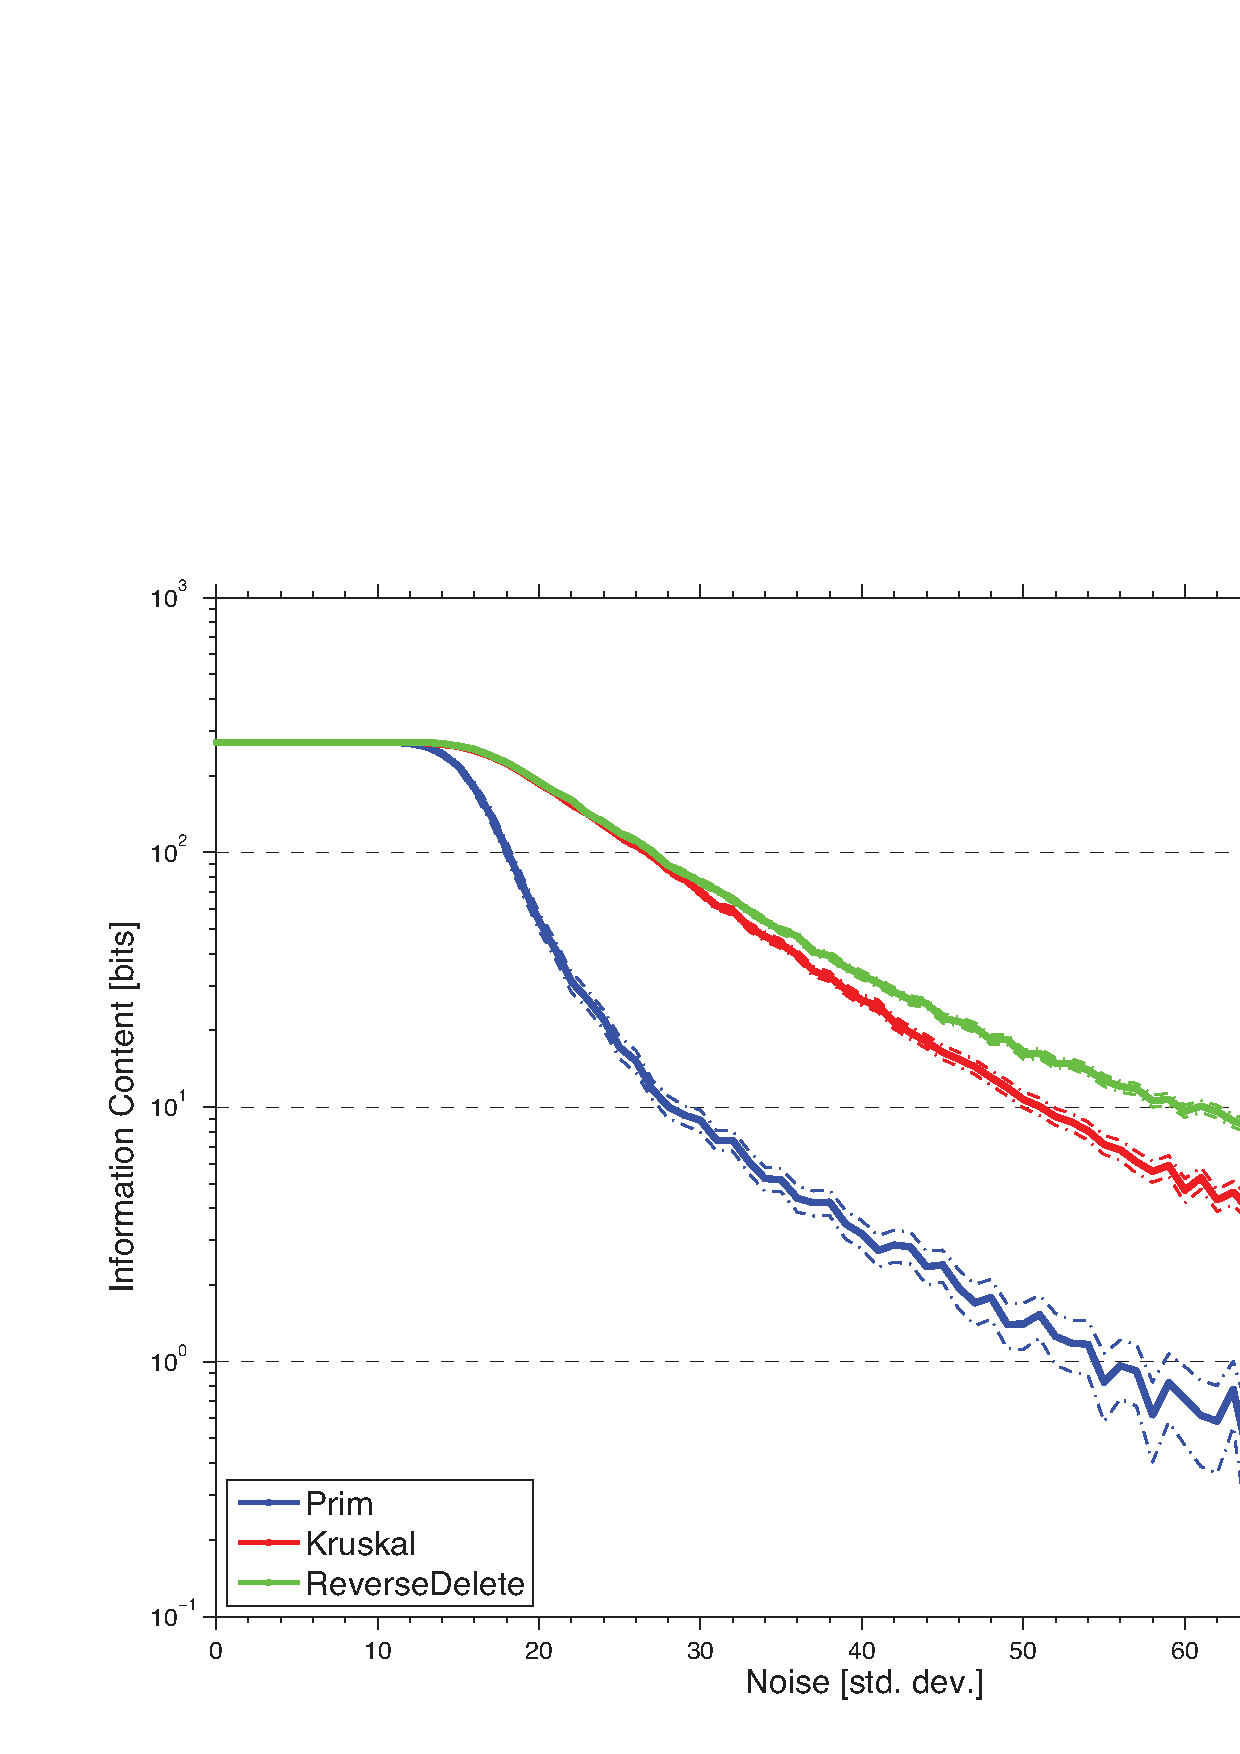
\includegraphics[width=.9\textwidth]{figures/ch_mst/gaus_inf_log}
\caption{Gaussian noise model: information content}
\label{fig:gaus_inf}
\end{figure}

\subsection{Experiment Setting: Gaussian Noise Model}
To investigate the general information-theoretic behavior of MST
algorithms in practice, we generate weighted complete graphs in a
hierarchical way. First, we generate a ``ground truth'' graph with
$n = 50$ vertices and with edges that are attributed by Gaussian weights,
sampled i.i.d. from a Gaussian distribution $\mathcal{N}(\mu_0 = 100,
\sigma_0^2 = 100)$.
Second, perturbed versions of this ground truth graph are then obtained by
adding Gaussian noise $\mathcal{N}(\mu = 0, \sigma^2)$ to the edge
weights for a given noise range $\sigma \in [0,  8\sigma_0]$.

In the experiment with approximation set-regularized algorithms we repeated the
experiment $400$ times to ensure the statistical significance of the
results. For some plots a semi-logarithmic scale was used for a better
visualization of small differences. Confidence intervals were also constructed
and plotted.

\subsection{Algorithmic Approximation Capacity Ranking of Algorithms}
\index{Ranking}
We plot the algorithmic information content $\max_t \Expct \hat
I_t^{\algo}(X', X'') $~(cf.~\eqref{eq:alg_eq:mst_asc_ratio}) for three algorithms (Figure~\ref{fig:gaus_inf}).
%%% JB: no new paragraph
At low noise levels (particularly $\sigma = 0$) all the three
algorithms exhibit the same information content, which is equal to
$\log_2{n^{n-2}} = 48 \log_2{50} \approx 270,9$ bits of information:
at zero noise, all the three algorithms choose the true MST out of
$|\C|$ possible spanning trees. For a complete graph,
Cayley's tree formula calculates the number of possible solutions as
$|\C| = n^{n-2}$.
%%% JB: In a noise-free setting, extracting the right tree corresponds
%%% to $\log_2{n^{n-2}} = 48 \log_2{50} \approx 270,9$ bits of
%%% information.    

The plot in Figure~\ref{fig:gaus_inf} provides a clear ranking of the three algorithms
w.r.t. their information content dependent on the noise level. A qualitative explanation 
which accounts for such ranking and 
clarifies the idea behind evaluating information content, is the
following:
%
%\begin{figure}[!t]
%\centering
%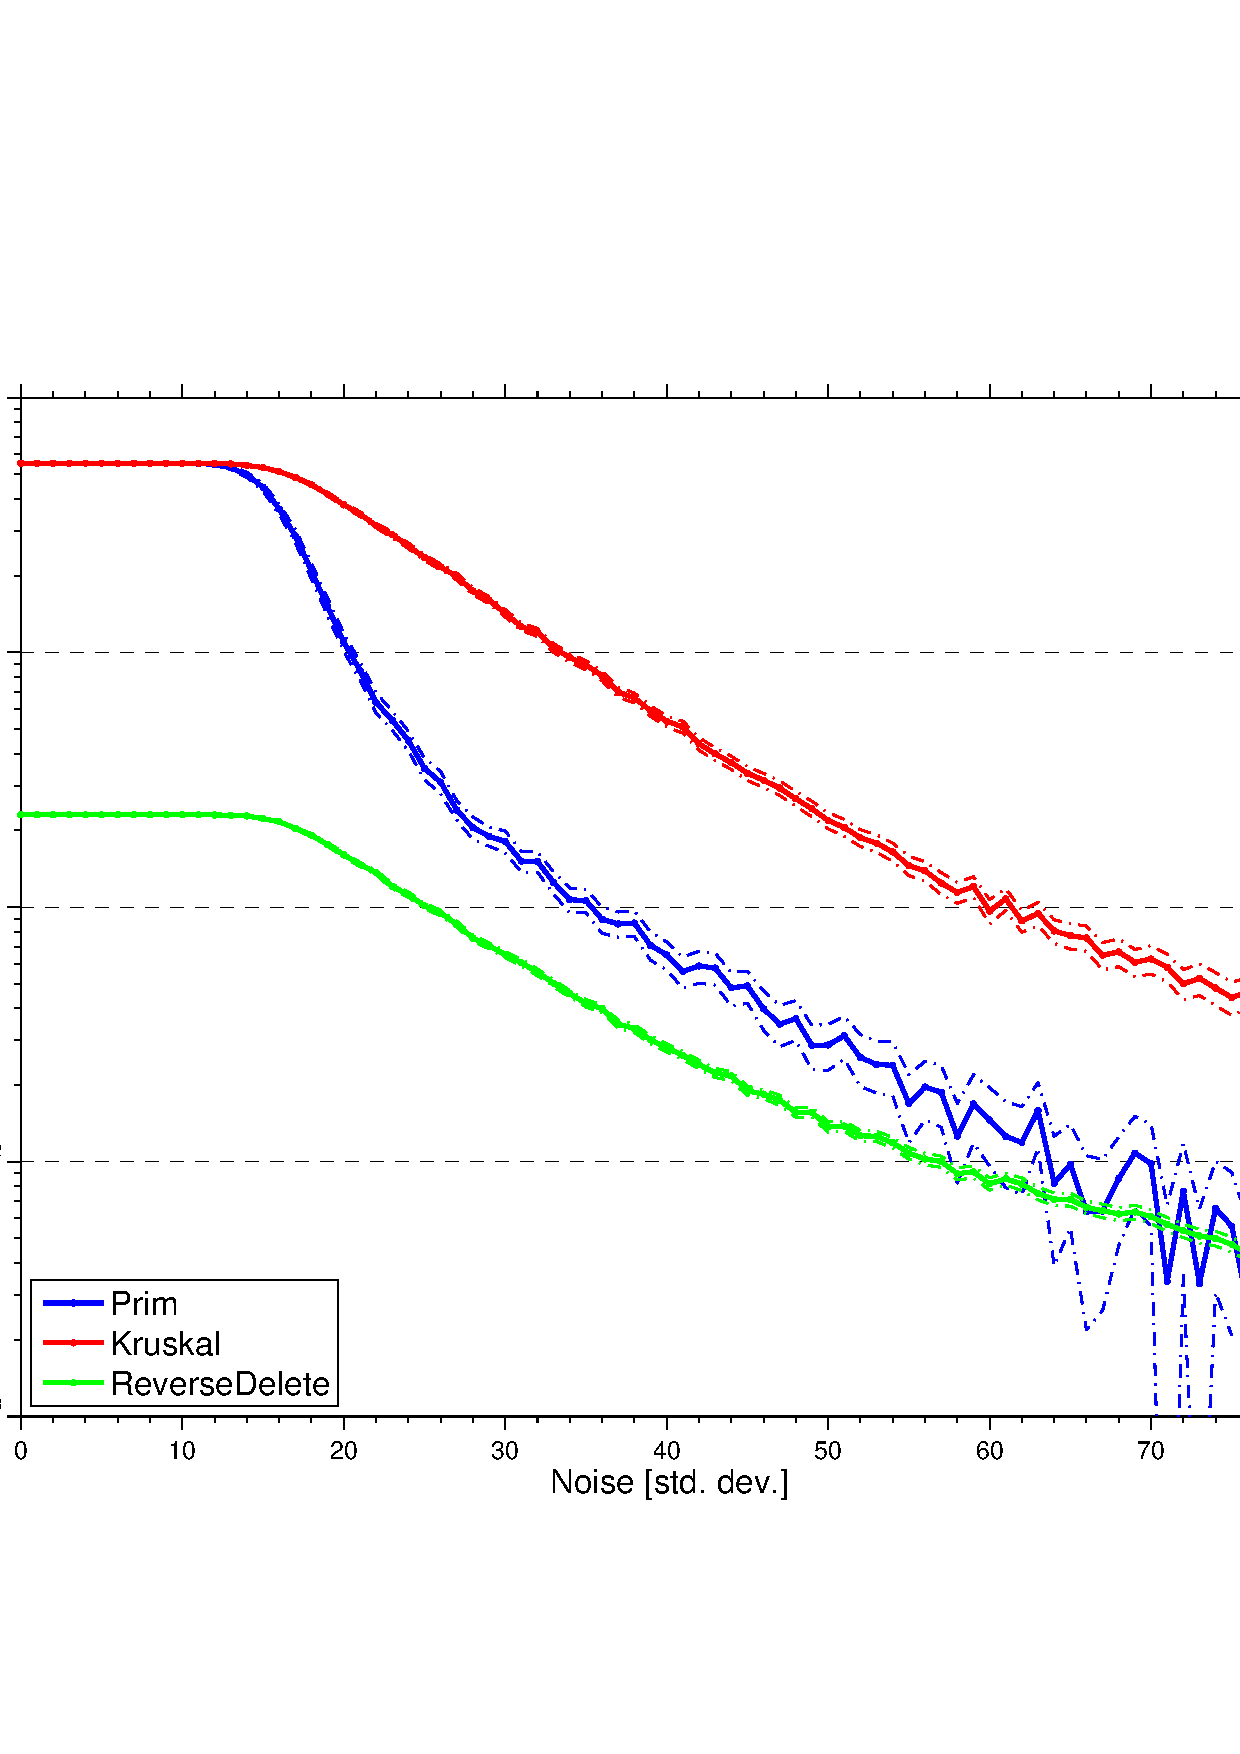
\includegraphics[scale=0.3]{figures/ch_mst/gaus_inf_step_log}
%\caption{Gaussian noise model: information content per step}
%\label{fig:gaus_inf_step_log}
%\end{figure}

\emph{Prim's algorithm} considers for addition only the edges which
are already connected to the tree built so far.  Among the not yet
considered edges there might be low cost edges which are more
efficient to be added in the beginning of the run rather than in the
end, thus making the information extraction inefficient from the point
of view of the algorithm dynamics.

\emph{Kruskal's algorithm} explores all the possible edges as
candidates for addition at each step, thus being less inclined to add
inefficient edges first and using the algorithm dynamics in a
efficient way. This gain is reflected by its increased informativeness
relative to Prim's algorithm.

\emph{Reverse-Delete algorithm} is more informative than Kruskal's,
since it efficiently discards all those edges which should not be
included in any approximate spanning tree. It pursues a strategy of
delayed decision making, that proved to be favourable also in other
situations of decision making under uncertainty.

\begin{figure}[!t]
\centering
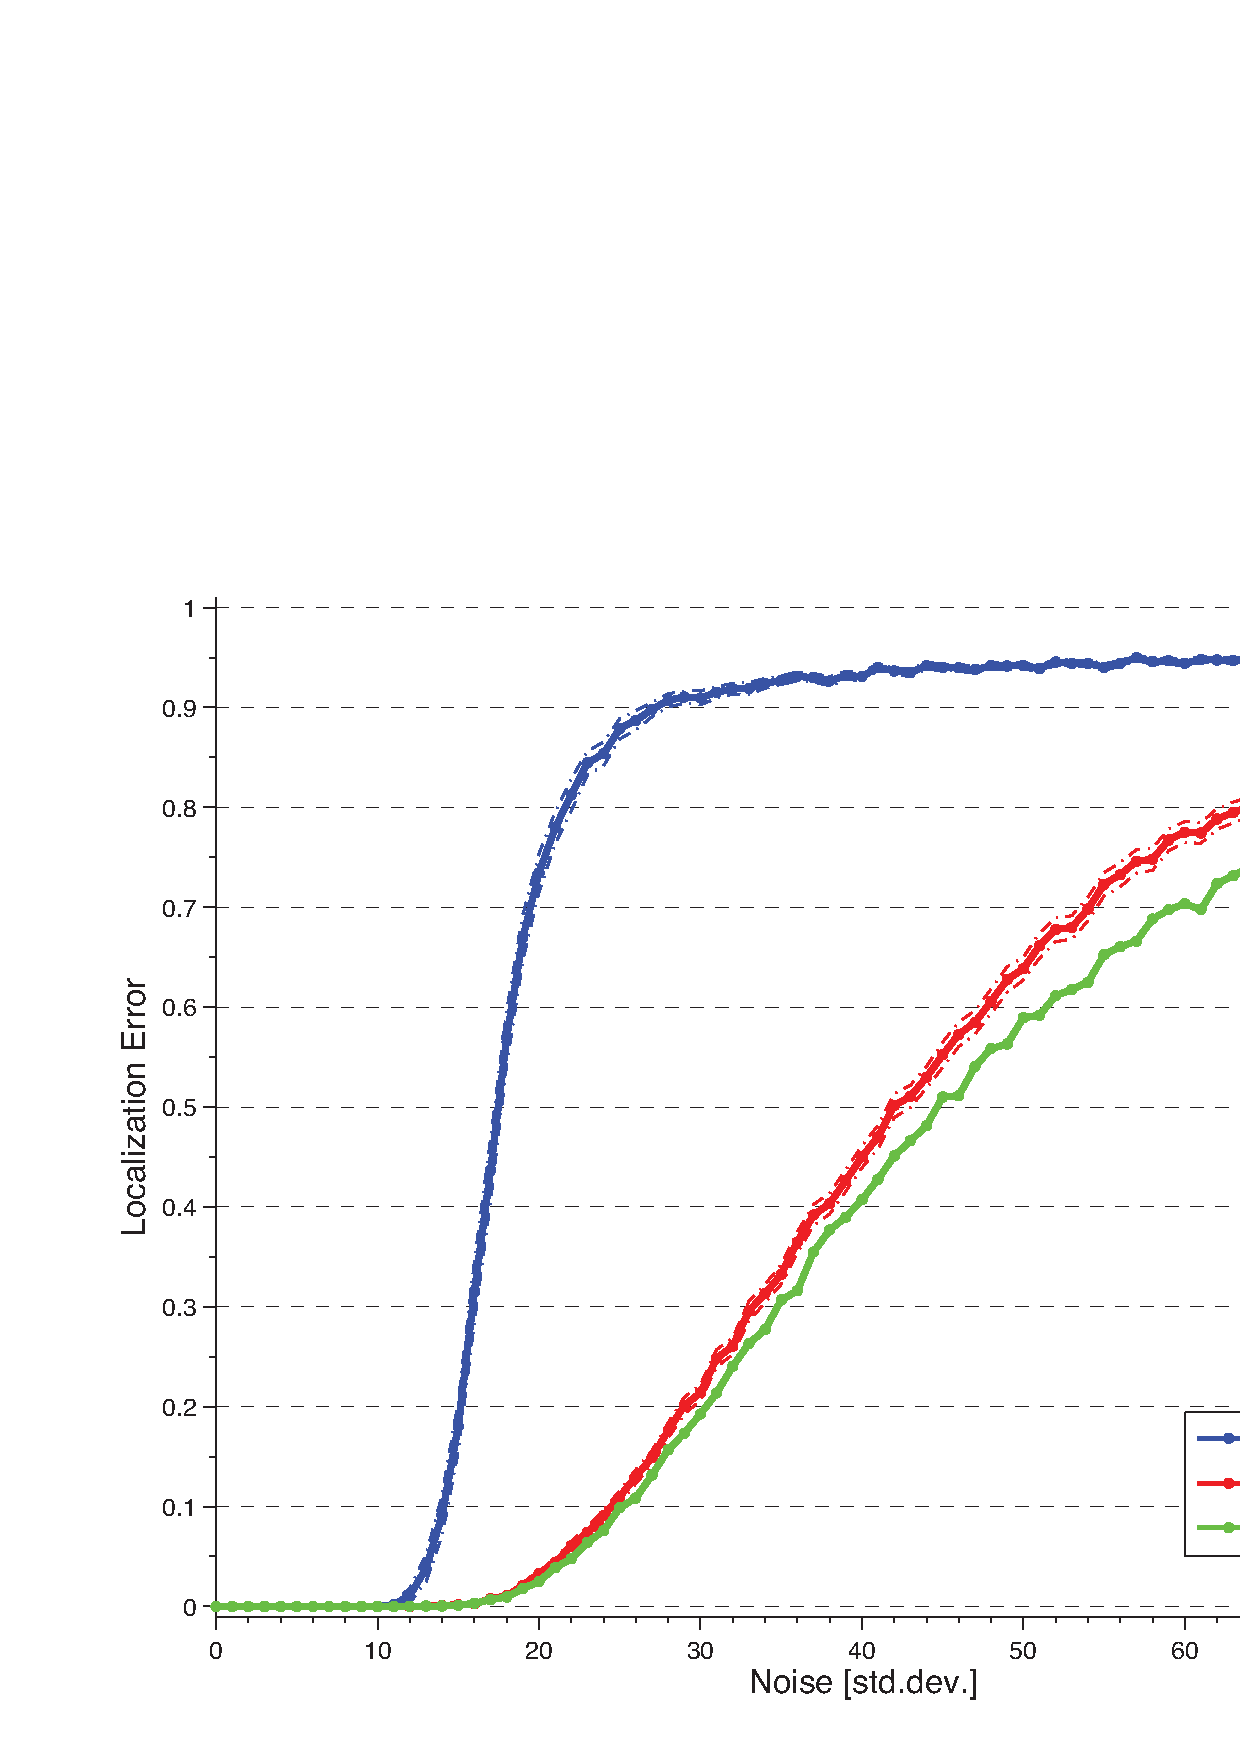
\includegraphics[width=0.9\textwidth]{figures/ch_mst/gaus_loc_err_mod}
\caption{Gaussian noise model: localization error}
\label{fig:gaus_loc_err}
\end{figure}

The above insights are proven by the plot showing the stepwise
dynamics of logarithm of the cardinalities $|\C^\algo_t(X')|$, $|\C^\algo_t(X'')|$
(Figure~\ref{fig:gaus_as_card}). It visualizes the
fact, that as $t$ progresses, Prim's algorithm contracts for the
solution faster than Kruskal's, and both contract faster that the
Reverse-Delete one, which, in turn, forces earlier stopping and thus
leads to the worse performance. In fact, we can formulate an informal statement:
\begin{statement}
  Assume that at the step $t$ the algorithm exhibits the edge set $B$ defined
  above in Section~\ref{sec:applying_asc_to_mst}. Then the reduction of the
  amount of feasible spanning trees with edges in $B$ obtained by adding
  $e_{t+1}$ which is adjacent to $B$  (Prim) is higher than the reduction
  obtained by adding non-adjacent $e_{t+1}$ (Kruskal in general), and both are
  higher than the reduction obtained by deleting $e_{t+1}$ from $B$
  (Reverse-Delete).
\end{statement}

\index{Stepwise dynamics}
The plot in the Figure~\ref{fig:gaus_ratio_dyn} explains the discussed ranking
from the stepwise dynamics prospective. The algorithm, which reaches maximum of
mutual information earlier, is less informative in overall, and vice versa. This
behavior reflects a natural trade-off between early decision and informativeness of the
solution.

\subsection{Localization Error Ranking of Algorithms}

\index{Ranking}
The three given algorithms ``explore'' the solution set with different
dynamic behavior, extracting different amount of the information
about the true solution. This behavior is related to the localization error.

For the algorithmically ASC-regularized
(Section~\ref{subsec:asc_regularization_crit}) solution $\hat c$
we plot (Figure~\ref{fig:gaus_loc_err}) the localization error, which is
computed as $E(\hat c) = 1 - |c^* \cap \hat c| / |c^*|$, where straight brackets
denote the cardinality of edges.

\begin{figure}[!t]
\centering
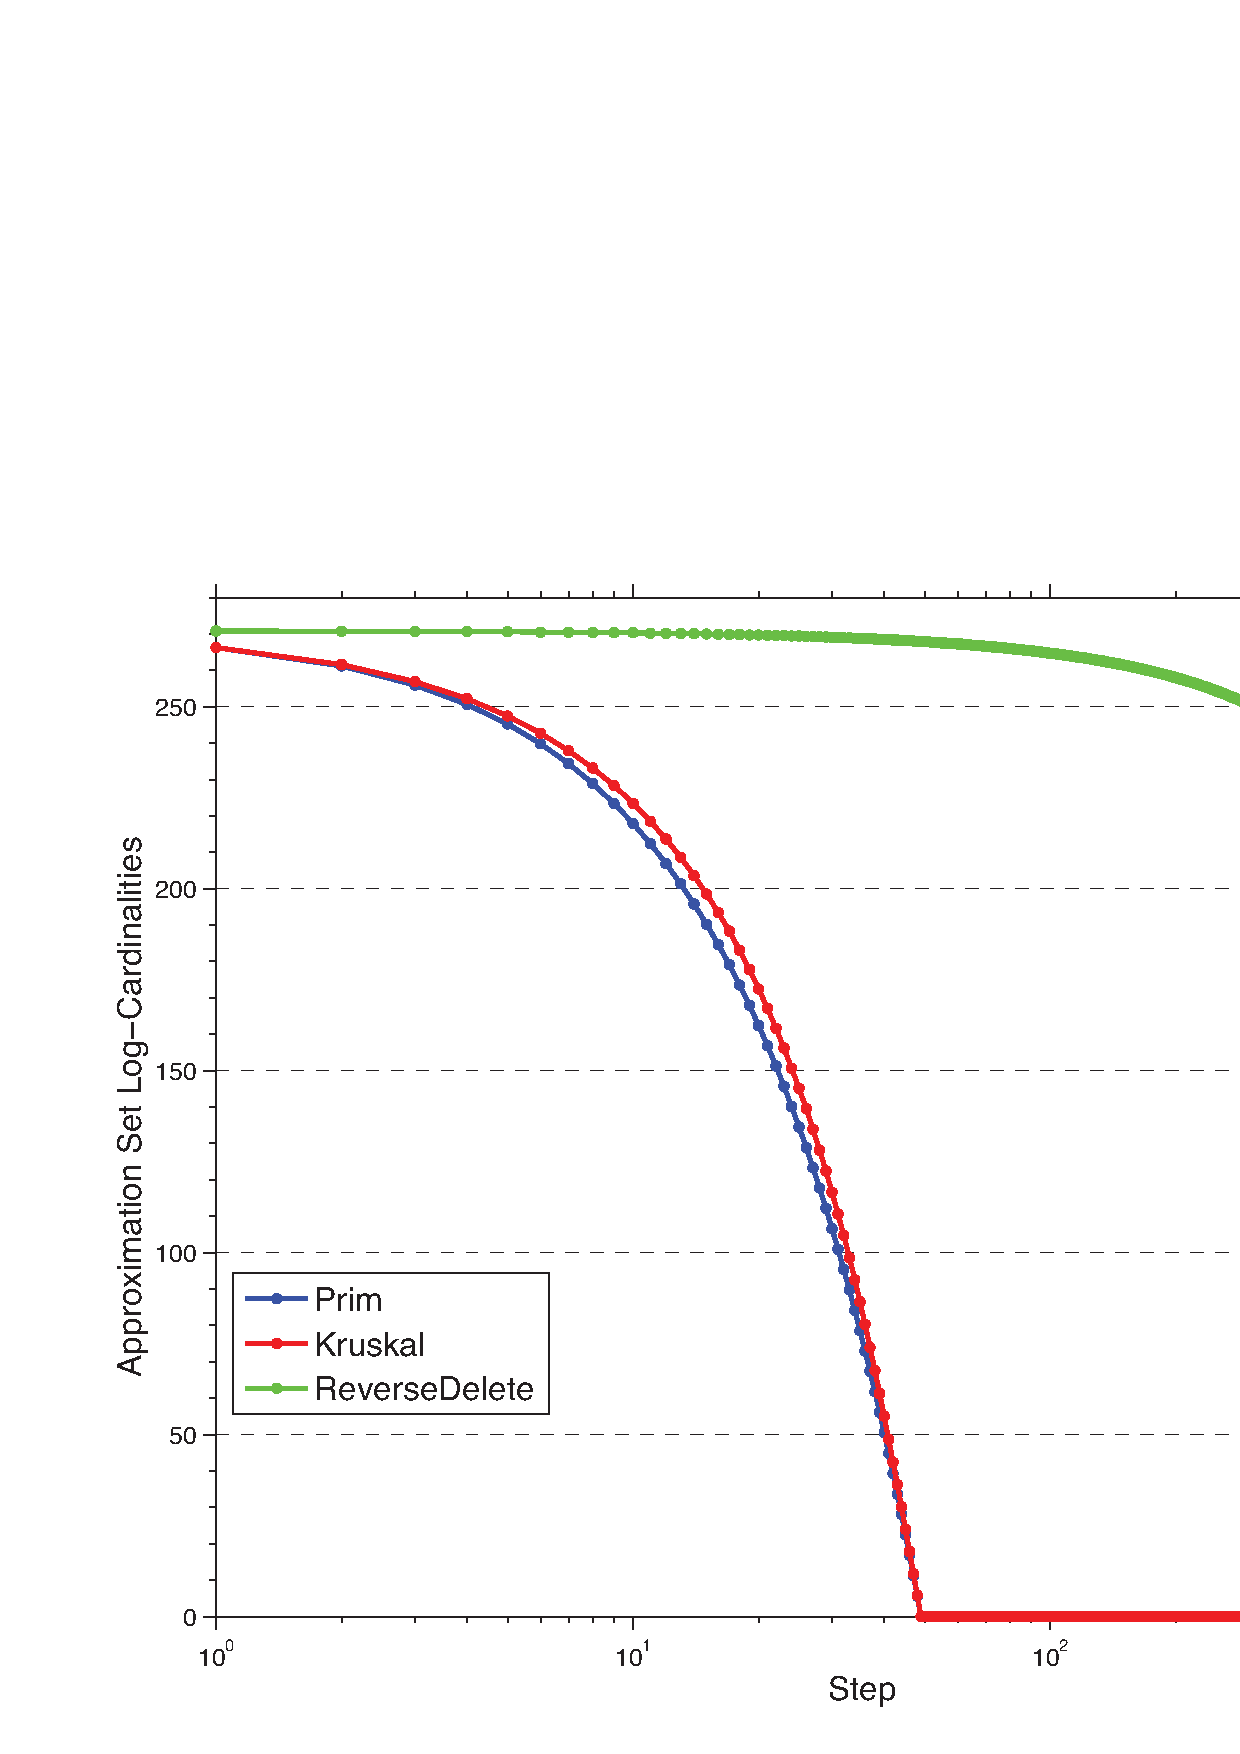
\includegraphics[width=.9\textwidth]{figures/ch_mst/gaus_as_card}
\caption{Gaussian noise model: stepwise approximation set log-cardinalities ($\sigma = 48$)}
\label{fig:gaus_as_card}
\end{figure}

\index{Localization error}
It can be seen from the figures, that the ranking of the three
algorithms according to their localization capability is in connection
with the information content ranking~--- the more informative
algorithm yields less error in localizing the true solution.

\begin{figure}[!t]
\centering
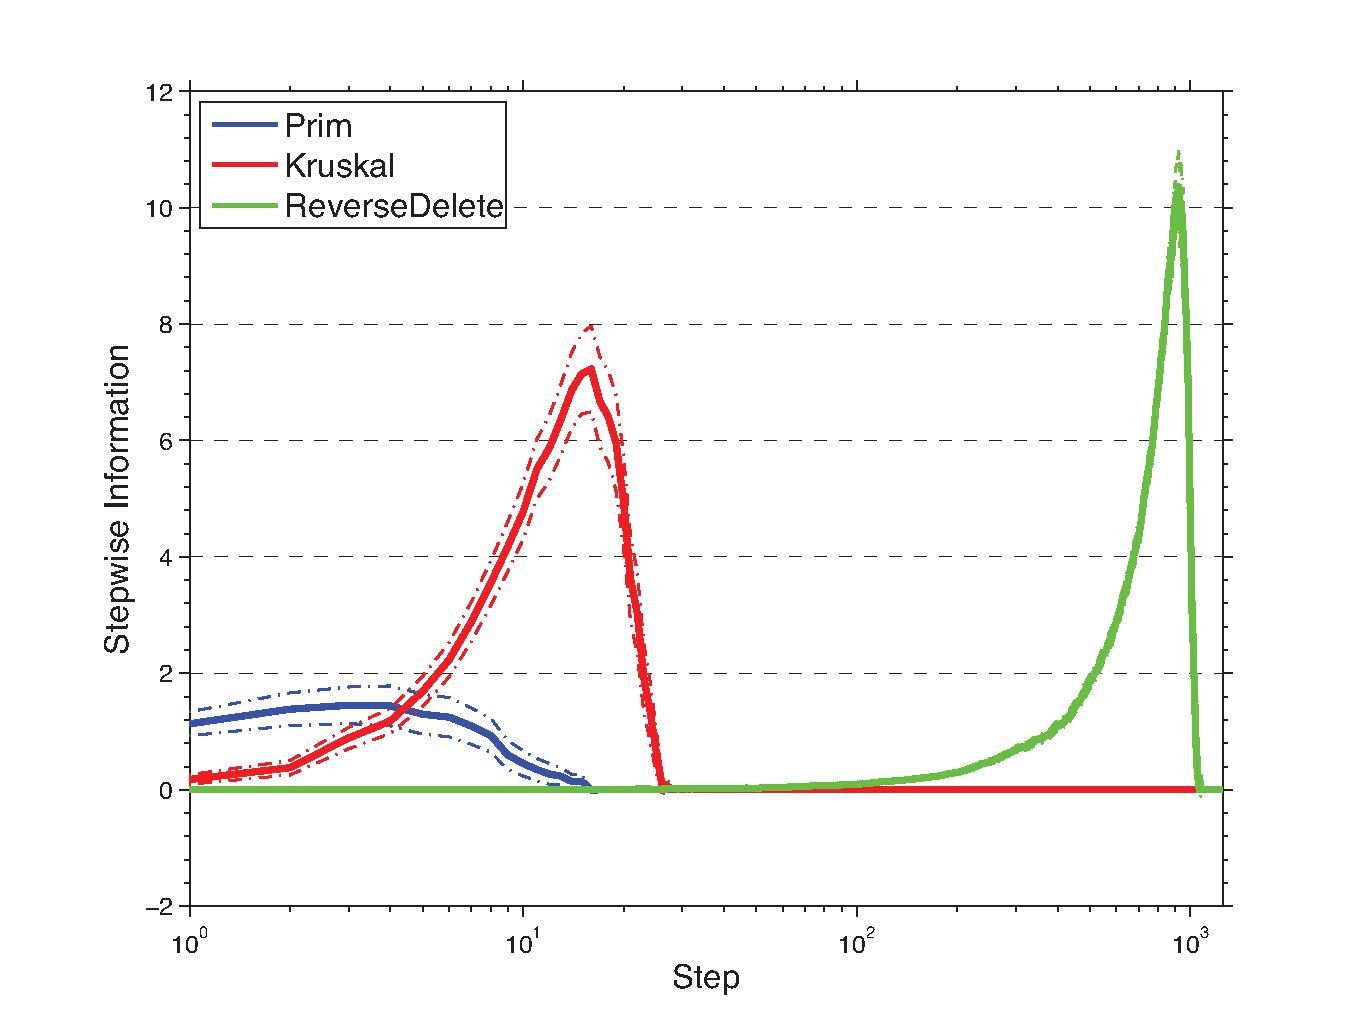
\includegraphics[width=.9\textwidth]{figures/ch_mst/gaus_ratio_dyn}
\caption{Gaussian noise model: stepwise algorithmic information defined in~\eqref{eq:alg_eq:mst_asc_ratio} ($\sigma = 48$)}
\label{fig:gaus_ratio_dyn}
\end{figure}
%
%\begin{figure}[!t]
%\centering
%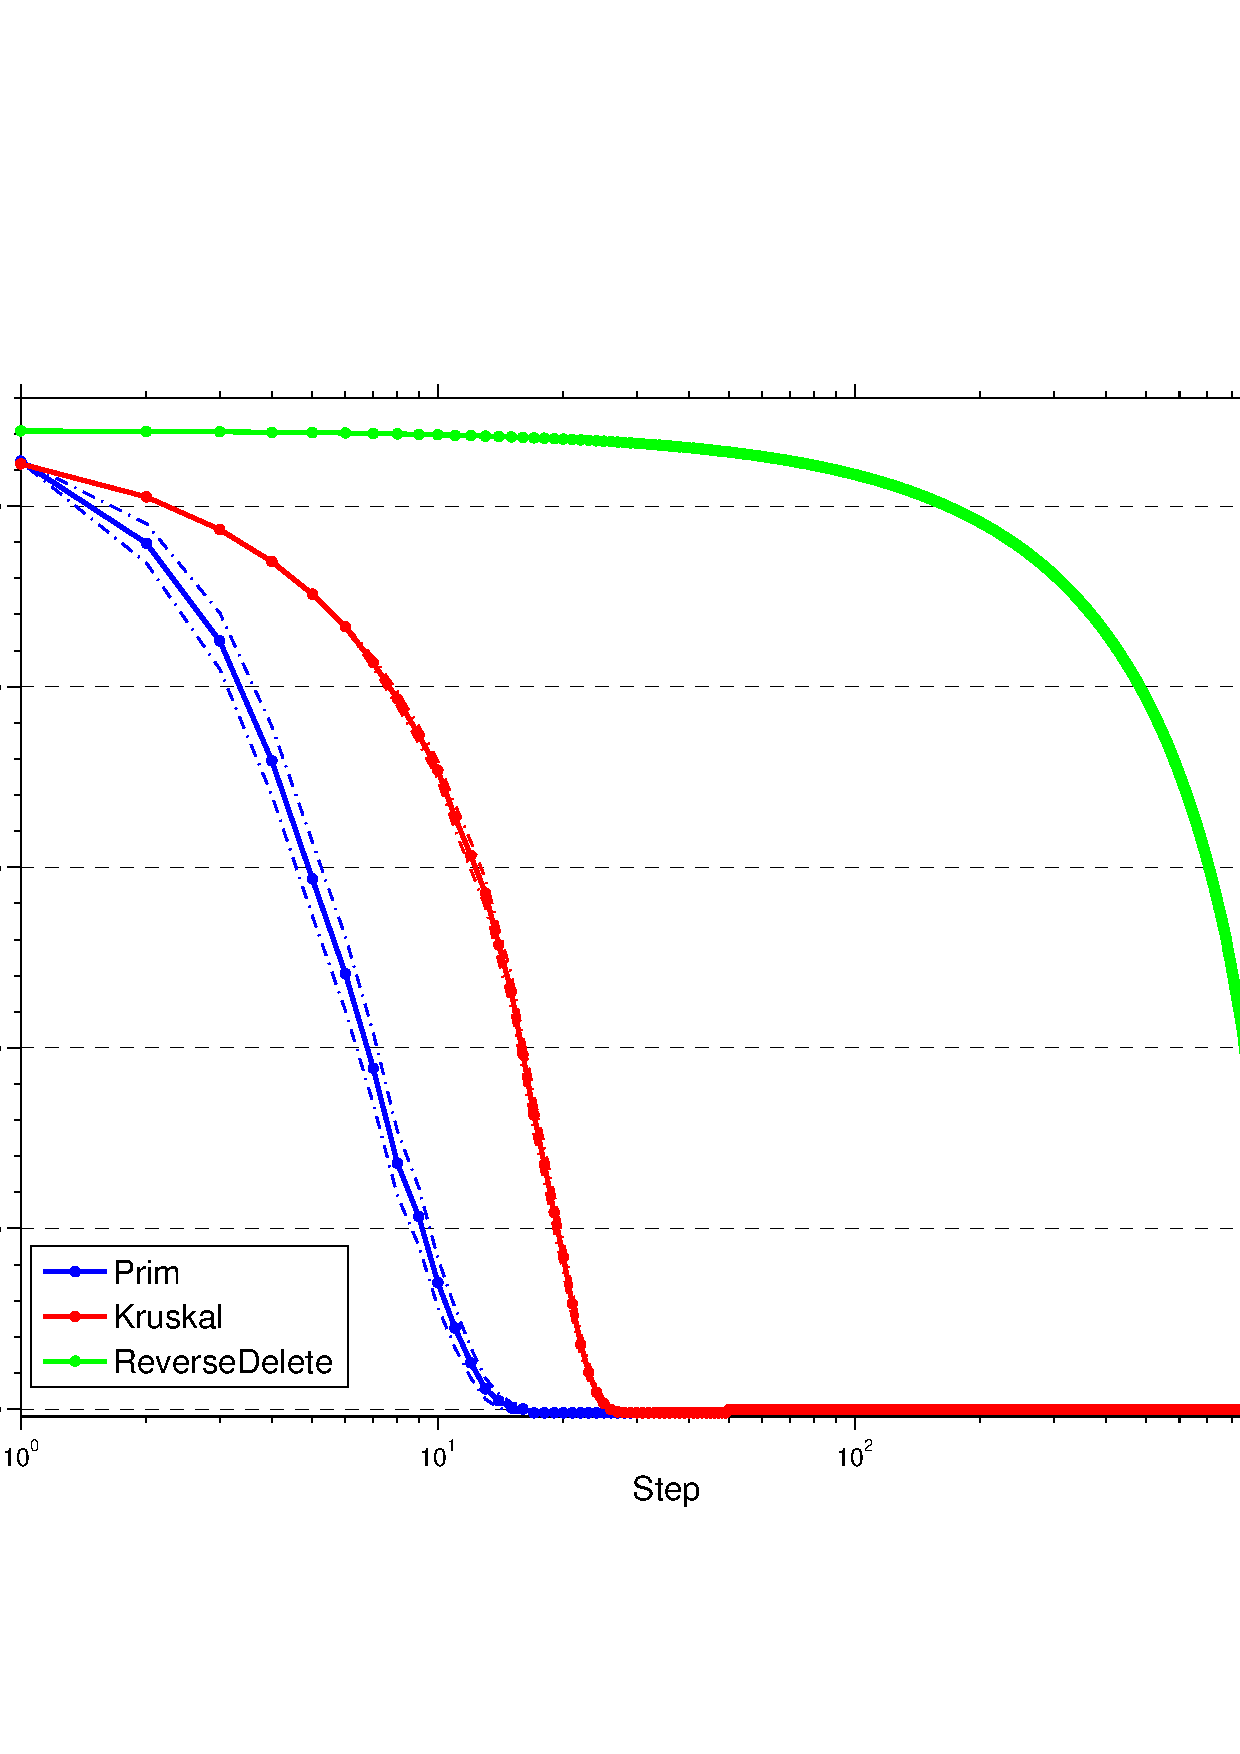
\includegraphics[scale=0.3]{figures/ch_mst/gaus_as_intersection_card}
%\caption{Gaussian noise model: stepwise approximation set intersection log-cardinalities ($\sigma = 48$)}
%\label{fig:gaus_as_intersect_card}
%\end{figure}

\subsection{Algorithmic ASC vs. Original ASC}
\label{sec:aasc_vs_asc}

As the last experiment, we showed that the original ASC regularization (the one
via $\gamma$-parameter) works still better than algorithmic ASC and even beats
the Joint Minimizer (first introduced as a benchmark solution in
Chapter~\ref{ch:gen_appch}), which minimizes the average cost $R(c, X')+R(c, X'')$.
\index{Joint cost minimizer}

Due to the computation limitations of the original ASC~--- it yields enumerating
the whole set of spanning trees ($n^{n-2}$) for each step $t$ --- we could only
run the experiments for graphs with few vertices ($n = 6$).
Figure~\ref{fig:aasc_vs_original} shows that the original ASC remains
competitive with the Joint Minimizer solution, while algorithmic version shows
weak performance. This is not surprising and comes at a certain cost for which
we discuss in conclusion.

\begin{figure}[!t]
\centering
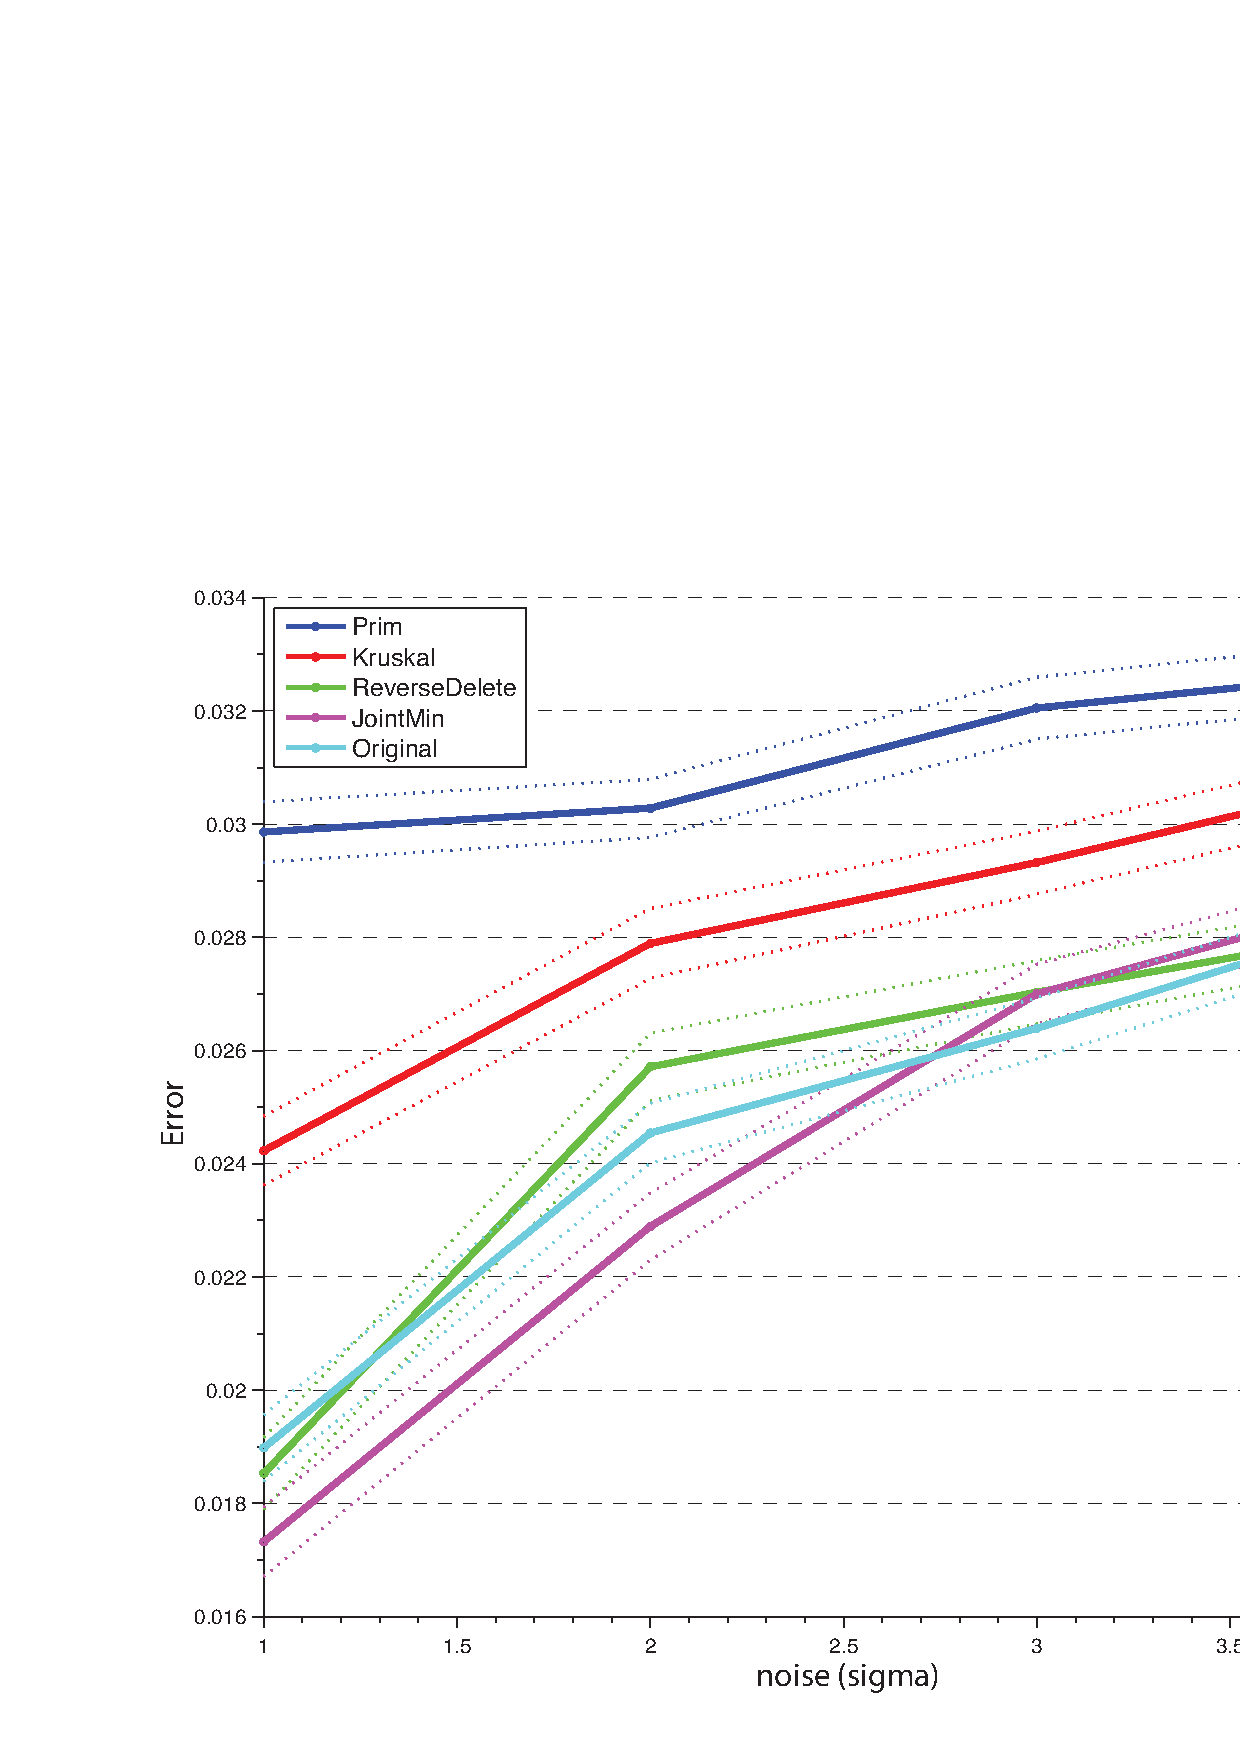
\includegraphics[width=.9\textwidth]{figures/ch_mst/gen_6_all}
\caption{Error plotted on the solutions obtained via original ASC
  (Chapter~\ref{ch:gen_appch} and algorithmic ASC (this chapter), as well as benchmarked on
  Joint Minimizer (Section~\ref{sec:aasc_vs_asc}).}
\label{fig:aasc_vs_original}
\end{figure}

\section{Discussion and Conclusion}
\label{sec:mst_conclusion}

\subsubsection{On the ASC-induced ranking of the algorithms}
The framework of approximation set coding is generalized from
the domain of models to the domain of algorithms in the
chapter. This framework enables us to apply an information-theoretic
regularization and quality assessment principle to algorithms,
and, in particular, to a minimum spanning tree problem with noisy
graphs as input.

We interpreted the results of the quantitative analysis of the
algorithms in a qualitative way, binding the strategy of the algorithm
to its information content, showing consistency and agreement with the
localization capability of the algorithm.

The ranking of the quantities plotted in
% Figure~\ref{fig:gaus_inf},~\ref{fig:gaus_loc_err},~
% \ref{fig:gaus_as_card},~ \ref{fig:gaus_ratio_dyn}
Figure~\ref{fig:gaus_inf}--\ref{fig:gaus_ratio_dyn}
support the following conjecture.
\begin{conj}
  The information content of contractive algorithms applied to the
  same problem establishes a ranking among them. This ranking is
  consistent with the average localization error of these algorithms.
\end{conj}

A possible way of investigating this relation is a rigorous analysis of the
approximation set dynamics using the mentioned Matrix-Tree theorem.
Although we utilized the simplest model of Gaussian noise,
independent on separate edges, there exists evidence, which
allows us to expect the same consistent results for a \emph{structured}
noise setting, when the edges of the graph are impacted by the noise
in a complex way, involving the statistical dependence of the noise
ingredients and other degrees of the noise model complexity.

\subsubsection{Algorithmic ASC vs. original ASC}

Should one use algorithmic approximation approach of this chapter or the
original $\gamma$-approximation approach form Chapter~\ref{ch:gen_appch}? In
this section, we address a question on whether the optimal stopping rule derived
by algorithmic ASC can compete with the original ASC (we initiated this discussion
in Section~\ref{sec:aasc_vs_asc}).

In fact, these two approaches serve quite different purposes and feature
different highlights. The original $\gamma$-parametrized ASC regularization
works in conjunction with the optimization goal $R(c, X)$, while its algorithmic
version makes use of algorithm-specific \textit{flow}. Although the algorithm
finds the same global optimizer as a bare $R(c, X)$-minimization procedure, the
structure of approximation sets if very different. Below, we list the main
points of difference:
\begin{itemize}
\item The original ASC relates to the continuous parameter, while algorithmic ASC
works with a discrete steps. This yields different power of resolution at which 
we coarse-grain the solution set $\C$. For original ASC, this resolution power 
is higher (it can allow much smaller step between approximation set sizes), while 
for algorithmic ASC it fully depends on the algorithm.

\item Original ASC is hard to apply computationally, since it boils down to 
computing and enumerating approximation sets. For algorithmic ASC, it is easier
to derive a problem-specific procedure which makes it \textit{orders of
magnitude} faster. For example, in the MST case, we utilized the Matrix-Tree
theorem and computed the cardinalities analytically at each step!
\end{itemize}

Hence, the trade-off between the power of resolution and the computational 
power exists and should be addressed in each special case.

\subsubsection{General notes on the ASC approach to algorithms}

From the statistical physics perspective, a contractive algorithm can be
considered as a process, where the temperature decreases step by step, and thus
``freezes'' the solution space, until finding the optimal solution. The
survey~\citep[Sec.~3.2]{Merhav:2010} discusses the connection between such a
coding framework and statistical physics. This connection \citep{JB:ISIT:2010}
inspires us to explore the dynamics of the algorithm from a generalization point
of view and to relate it to the information theory~\citep{Merhav:2010}.

We will consider the statistical physics viewpoint on the ASC regularization in the next
chapter.